% !TEX root = thesis.tex
%%%%%%%%%%%%%%%%%%%%%%%%%%%%%%%%%%%%%%%%%%%%%%%%%%%%%%%%%%%%%%%%%%%%%%%%%%%%%%%%
\chapter{Проектирование архитектуры инструментальной среды}
%%%%%%%%%%%%%%%%%%%%%%%%%%%%%%%%%%%%%%%%%%%%%%%%%%%%%%%%%%%%%%%%%%%%%%%%%%%%%%%%

\todo{В начале каждого раздела приводится краткое содержание. В конце вывод.}

%%%%%%%%%%%%%%%%%%%%%%%%%%%%%%%%%%%%%%%%%%%%%%%%%%%%%%%%%%%%%%%%%%%%%%%%%%%%%%%%
\section{Структура программной системы}
\label{sec:architecture}
%%%%%%%%%%%%%%%%%%%%%%%%%%%%%%%%%%%%%%%%%%%%%%%%%%%%%%%%%%%%%%%%%%%%%%%%%%%%%%%%

\todo{Написать причины именно такой архитектуры}

На основе анализа поставленных требований, а также уже существующих решений,
была предложена следующая архитектура программной системы:

\begin{figure}[th]
    \begin{center}
        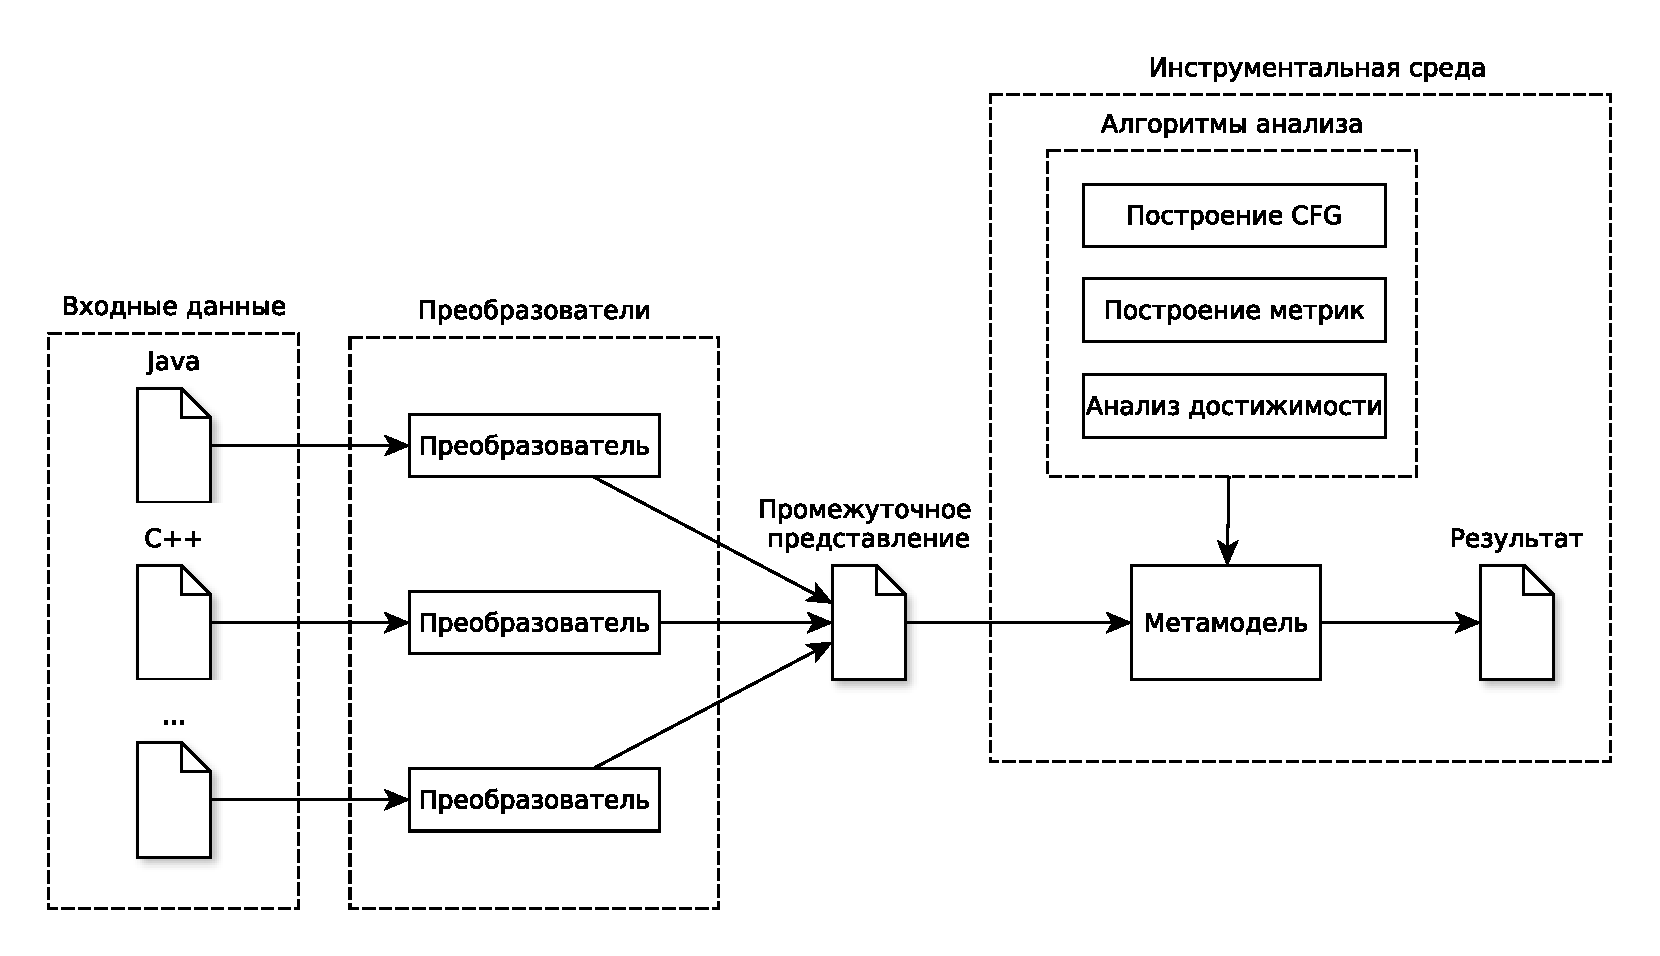
\includegraphics[width=\textwidth]{architecture.eps}
    \end{center}
    \caption{Архитектура программной системы}
    \label{fig:architecture}
\end{figure}

Как видно из рис.~\ref{fig:architecture} система состоит из 3-х частей:

\begin{enumerate}
    \item Центральная часть системы - \emph{метамодель}. Над ней производятся
    все операции по проведению анализа и графического отображения свойств
    анализируемой системы.
    \item \emph{Преобразователи} отвечают за импортирование исходного кода
    анализируемой системы и его преобразование в промежуточное представление
    (сериализованную метамодель). Преобразователи являются единственной частью
    системы, зависящей от языка программирования, на котором написана
    анализируемая система. Однако, так как инструментальная среда оперирует
    только с промежуточным представлением, то преобразователи могут поставляться
    сторонними разработчиками, тем самым избавляя программиста от необходимости
    поддерживать все возможные языки.
    \item \emph{Процедуры анализа} вместе с \emph{метамоделью} являются
    ключевыми составляющими инструментальной среды. Инструментальная среда
    содержит графический интерфейс пользователя, на котором в том или ином виде
    отображается результат проведенного анализа.
\end{enumerate}

%%%%%%%%%%%%%%%%%%%%%%%%%%%%%%%%%%%%%%%%%%%%%%%%%%%%%%%%%%%%%%%%%%%%%%%%%%%%%%%%
\section{Проектирование метамодели}
\label{sec:metamodel_architecture}
%%%%%%%%%%%%%%%%%%%%%%%%%%%%%%%%%%%%%%%%%%%%%%%%%%%%%%%%%%%%%%%%%%%%%%%%%%%%%%%%
Существует два подхода к разработке метамодели:

\begin{enumerate}
    \item Разработка архитектуры ``с нуля''
    \item Использование стандартных средств описание метамоделей, т.н.
    мета-метамоделей.
\end{enumerate}

Каждый из двух подходов обладает своими достоинствами и недостатками, а именно:

\begin{enumerate}
    \item Собственная метамодель позволит сильно упростить ее структуру,
    специализировав ее под нужды инструментальной среды, что увеличит
    производительность разрабатываемых алгоритмов над метамоделью и облегчит ее
    использование. Однако данный подход обладает очень высокими рисками, так как
    данная составляющая является ключевой в разрабатываемой среде, и ошибки в ее
    проектировании могут привести к провалу проекта.
    \item Использование стандартных средств менее подвержено рискам, но, в силу
    универсальности данного подхода, получившаяся метамодель может быть слишком
    громоздкой в использовании.
\end{enumerate}

В результате анализа было принято решение об использовании стандартной
архитектуры, но с незначительными изменениями, чтобы скомбинировать достоинства
обоих подходов к проектированию.

\subsection{Стандарт MOF}

Рассмотрим подробнее существующий стандарт разработки метамоделей:

\nomenclature{OMG}{Object Management Group, консорциум, занимающийся разработкой
и продвижением объекто-ориентированных технологий и стандартов}
\nomenclature{UML}{Unified Modeling Language, унифицированный язык моделирования}
\nomenclature{MOF}{Meta-Object Facility, стандарт для разработки, управляемой моделями}
\nomenclature{MDE}{Model-Driven Engeneering, разработка, управляемая моделями}
\nomenclature{MDA}{Model-Driven Architecture, подход к разработке программных систем}
\nomenclature{РБНФ}{Расширенная Форма Бэкуса-Наура}

В 1997 году группой OMG был создан унифицированный язык моделирования (UML).
UML позволяет описывать различные компоненты и артефакты системы, тем
самым упрощая процесс разработки~\cite{Fowler03}.

Для описания конструкций языка UML был разработан фреймворк MOF (Meta Object
Facility)~\cite{mof}. В дальнейшем обе эти концепции вошли в подход, называемый
Model Driven Architecture (MDA)~\cite{miller2003}. Данный подход к разработке ПО
вводит дополнительный уровень абстракции, позволяющий описывать структуру и
поведение разрабатываемой системы, не завися от нижележащей используемой
технологии.

Таким образом, MOF является мета-метамоделью для описания метамоделей (например,
метамодели UML). Аналогично расширенной форме Бэкуса-Наура (РБНФ), которая
задает грамматику языка программирования, MOF позволяет задавать структуру и
абстрактный синтаксис метамодели.

На данный момент последней версией стандарта является версия 2.4.2, выпущенная в
2014 году~\cite{mof}.

\subsection{Иерархия моделей MOF}

Архитектура MOF определена в контексте иерархии моделей, на верхнем уровне
которой и находится MOF. Данная иерархия выглядит следующим образом:

\begin{description}
    \item[M3] - слой мета-метамоделей
    \item[M2] - слой метамоделей
    \item[M1] - слой моделей
    \item[M0] - слой времени исполнения
\end{description}

Слои M3 и M2 так же называются \emph{слоями спецификации
языков}~\cite{essay57286}. Каждый слой является уровнем абстракции - чем ниже
слой, тем конкретнее описывается система.

На слое M3 находится только одна метамодель - MOF,
задача которой - описание метамоделей. На уровне M2 располагается множество
метамоделей, которые являются экземплярами MOF. Слой моделей
содержит пользовательское описание системы. Слой M0 содержит объекты системы во
время ее исполнения.

Ниже приведен пример иерархии для конкретной системы:

\begin{figure}[ht]
    \begin{center}
        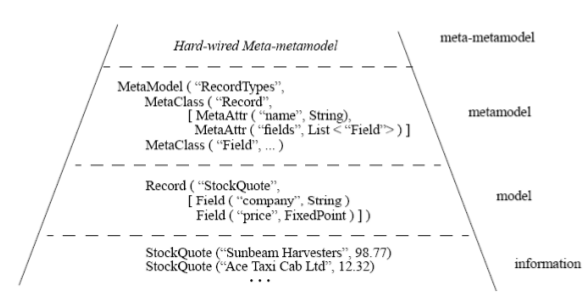
\includegraphics[width=\textwidth]{hierarchy_example.png}
    \end{center}
    \caption{Пример иерархии моделей}
    \label{fig:model_hierarchy}
\end{figure}

Теоретически, иерархию можно дополнить дополнительными слоями над слоем M3,
однако MOF позволяет рекурсивно описывать вышележащие слои, поэтому слои выше M3
не имеют смысла, так как содержат в себе ту же самую мета-метамодель.

\subsection{Структура MOF}

MOF обладает модульной структурой, каждый модуль называется \emph{пакетом}.
Пакеты можно так же объединять в пакеты, образуя иерархию пакетов. Существует
два пакета верхнего уровня - \texttt{MOF} и \texttt{UML infrastructure library}.

Стоит отметить, что MOF использует те же понятия для описания сущностей, что и
UML, таким образом, между пакетами образуется следующий вид отношения:

\begin{figure}[ht]
    \begin{center}
        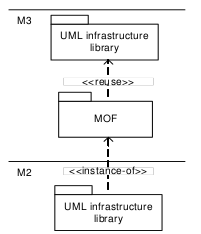
\includegraphics[width=0.4\textwidth]{mof_packages.png}
    \end{center}
    \caption{Взаимосвязь между пакетами MOF верхнего уровня}
    \label{fig:mof_packages}
\end{figure}

Данные пакеты включают в себя множество подпакетов, дерево которых приведено
на рис.\ref{fig:mof_packets}:

\begin{figure}[ht]
    \begin{center}
        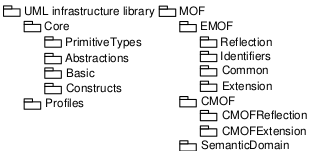
\includegraphics[width=0.6\textwidth]{mof_packets.png}
    \end{center}
    \caption{Дерево пакетов MOF}
    \label{fig:mof_packets}
\end{figure}

Опишем некоторые из приведенных пакетов:

\todo{Добавить везде слово Пакет в названиях}

\subsubsection{Abstractions}

Данный пакет содержит элементы, которые затем используются во всех других
пакетах. В нем содержатся такие элементы как выражения, литералы,
пространства имен, отношения и т.д.

\subsubsection{Basic}

Пакет Basic предназначен исключительно для облегчения использования и объединяет
в себе сущности из нескольких других пакетов.

\subsubsection{Constructs}

В данном пакете содержатся конкретные экземпляры классов из пакета Abstractions,
например, классы различных отношений, конструкций языка и т.д.

\subsubsection{EMOF}

\nomenclature{EMOF}{Essential MOF, базовая структурная составляющая MOF}

EMOF является объединяет в себе базовые концепции MOF, такие как Reflection
(возможность доступа к свойствам описываемого объекта), Element (базовая единица
метамодели, являющаяся экземпляром какого-либо класса), Common (пакет,
поддерживающий коллекции экземпляров Element).

Структура данного пакета приведена на рис.~\ref{fig:emof}:

\begin{figure}[ht]
    \begin{center}
        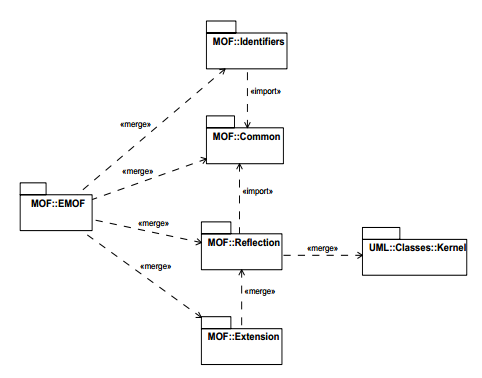
\includegraphics[width=0.8\textwidth]{emof.png}
    \end{center}
    \caption{Структура EMOF}
    \label{fig:emof}
\end{figure}

\subsubsection{CMOF}

\nomenclature{CMOF}{Complete MOF, основная структурная составляющая MOF}

Данный пакет включает в себя пакет EMOF с некоторыми дополнениями  (например, он
расширяет пакет Reflection, добавляя в него новые операции над сущностями).

На рис.~\ref{fig:circuit_mof} приведен краткий пример MOF-совместимой метамодели
для описания электрических схем~\cite{essay57286}:

\begin{figure}[ht]
    \begin{center}
        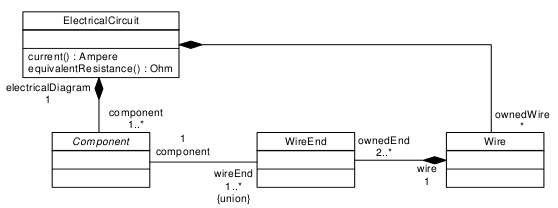
\includegraphics[width=\textwidth]{circuit_mof.png}
    \end{center}
    \caption{Метамодель для описания электрических схем}
    \label{fig:circuit_mof}
\end{figure}

Класс \texttt{Component} является базовым классом для всех сущностей, включая
\texttt{ElectricalCircuit}, которая отображает саму электрическую схему. Класс
\texttt{Wire} показывает вид отношений между объектами электрической схемы.

\subsection{Сериализация метамодели}

\nomenclature{XMI}{XML Metadata Interchange, формат для сериализации метамоделей
в формат XML}
\nomenclature{DTD}{Document Type Definition, описание схемы документа для языка разметки}

Для сериализации UML моделей и их передачи между различными средствами OGM был
разработан формат XMI. Но так как UML является совместимой со стандартом MOF,
XMI может быть использован для сериализации любой MOF-совместимой
метамодели~\cite{standard/XMI}.

В стандарт XMI входят следущие составляющие:

\begin{enumerate}
    \item Набор правил DTD для отображения метамоделей в XML документ
    \item Правила описания метаданных
    \item Схему XML для XMI документов
\end{enumerate}

Пример отношения между системой на языке программирования, ее модели и сериализованной
модели в XMI приведен на рис.~\ref{fig:xmi_example}:

\begin{figure}[ht]
    \begin{center}
        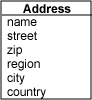
\includegraphics[width=0.8\textwidth]{xmi_example.png}
    \end{center}
    \caption{Отношение между MOF и XMI}
    \label{fig:xmi_example}
\end{figure}

Приведем пример сериализованной UML модели в формате XMI:

\begin{figure}[ht]
    \begin{center}
        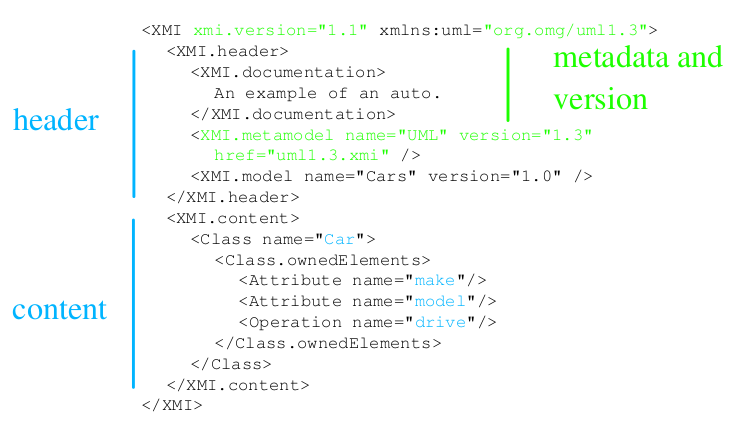
\includegraphics[width=0.8\textwidth]{xmi_document.png}
    \end{center}
    \caption{Пример сериализованной UML-модели}
    \label{fig:xmi_document}
\end{figure}

Таким образом, выбранный формат данных естественным образом ложится на
разработанную архитектуру, а его стандартизированность облегчает взаимодействие
между инструментальной средой и сторонними преобразователями. Это является
неоспоримым преимуществом по сравнению с другими форматам (JSON, формат
сериализации объектов JAVA и т.д.).

%%%%%%%%%%%%%%%%%%%%%%%%%%%%%%%%%%%%%%%%%%%%%%%%%%%%%%%%%%%%%%%%%%%%%%%%%%%%%%%%
\section{Проектирование архитектуры преобразователей}
\label{sec:transformer_architerture}
%%%%%%%%%%%%%%%%%%%%%%%%%%%%%%%%%%%%%%%%%%%%%%%%%%%%%%%%%%%%%%%%%%%%%%%%%%%%%%%%

Задача преобразователей - отображение исходного кода программы в метамодель.
Таким образом каждый преобразователь - это транслятор языка программирования, на
котором написана анализируемая программа.

Как и любой транслятор, преобразователь может иметь несколько фаз
выполнения~\cite{Aho1986}:

\begin{enumerate}
    \item Лексический анализ - выделение лексем во входном тексте программы
    \item Синтаксический анализ - построение синтаксического дерева по входному
    набору лексем в соответствии с грамматикой языка
    \item Семантический анализ - проверка семантических условий языка (например,
    соответствие типов, наличие объявления используемой переменной и т.д.)
    \item Оптимизация - преобразование промежуточного представления программы
    с целью повышения производительности, уменьшения размера генерируемого кода,
    объема используемой памяти и т.п.
    \item Генерация кода - получение результата выполнения трансляции
\end{enumerate}

Так как задачей преобразователя является генерация метамодели, некоторые фазы не
являются необходимыми (например, фаза оптимизации). Также, можно опустить фазу
семантического анализа, что сильно упростит код преобразователя, но скажется на
его простоте использования, так как пользователю будет необходимо проверять
корректность анализируемой системы сторонними средствами (например, при помощи
компилятора языка программирования, на котором написана анализируемая система).

Получившаяся структура преобразователя изображена на рис.~\ref{fig:translator}.

\begin{figure}[ht]
    \begin{center}
        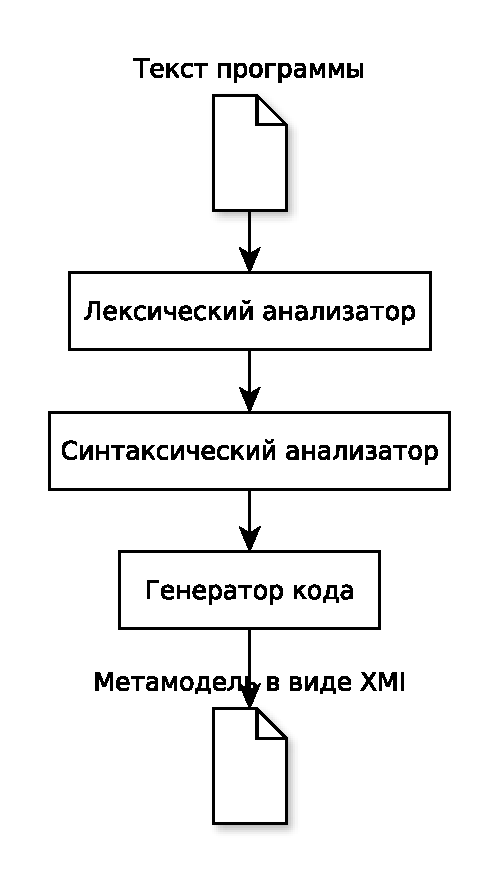
\includegraphics[width=0.4\textwidth]{translator.eps}
    \end{center}
    \caption{Архитектура преобразователя}
    \label{fig:translator}
\end{figure}

Существует два подхода к построению лексических (лексеров) и синтаксических
(парсеров) анализаторов:

\begin{enumerate}
    \item Написание кода лексера и парсера вручную (например, парсеров,
    использующие метод рекурсивного спуска или метод функциональных
    комбинаторов).
    \item Использование генераторов парсеров (например, табличных парсеров)
\end{enumerate}

К достоинствам первого метода можно отнести повышенное быстродействие,
пониженную ресурсоемкость и меньший объем кода лексера и парсера. К недостаткам
данного метода можно отнести высокую трудоемкость и сложность написания.

Использование генераторов парсеров значительно упрощает написание, тем самым
уменьшая количество возможных ошибок и дефектов. Однако сгенерированные парсеры
обладают худшей производительностью и предъявляют повышенные требования к объему
используемой памяти.

На основе анализа достоинств и недостатков обоих методов, было принято решение
об использовании автоматической генерации кода парсеров и лексеров
разрабатываемых преобразователей. В случае нехватки производительности или
объема предоставляемой памяти по результатам профилирования возможна разработка
новых преобразователей с использованием вручную написанных парсеров и лексеров.

Результатом работы преобразователя является сериализованная метамодель в формате
XML. Так как структура XML-файла полностью отражает структуру метамодели, для ее
сериализации рационально использовать различные фреймворки для преобразования
объектов программы в формат XML.

%%%%%%%%%%%%%%%%%%%%%%%%%%%%%%%%%%%%%%%%%%%%%%%%%%%%%%%%%%%%%%%%%%%%%%%%%%%%%%%%
\section{Проектирование графического интерфейса}
%%%%%%%%%%%%%%%%%%%%%%%%%%%%%%%%%%%%%%%%%%%%%%%%%%%%%%%%%%%%%%%%%%%%%%%%%%%%%%%%

При проектировании графической составляющей инструментальной среды необходимо
решить следующие проблемы:

\begin{enumerate}
    \item Унификация процедур анализа над метамоделью для обеспечения
    возможности добавления новых процедур по мере необходимости
    \item Удобство отображения моделей сложных программных систем
\end{enumerate}

Так как большинство процедур анализа строится на обходе структуры метамодели, то
для решения первой проблемы целесообразно применить паттерн ``Посетитель''
(Visitor)~\cite{Gamma94}. Применение данного паттерна позволит абстрагировать
метамодель от алгоритмов над ней, выделив обход ее структуры в отдельный класс.

Необходимые виды визуализации, описанные в п.~\ref{sec:task}, имеют вид дерева
или графа, поэтому для решения второй проблемы можно применить следующие способы
уменьшения размера отображаемой модели системы:

\begin{enumerate}
    \item Сворачивание отдельных узлов и примыкающих к ним дуг
    \item Масштабирование всего графа относительно размера панели отображения
    визуализаций
\end{enumerate}
